\documentclass[a4paper]{book}
%\documentclass[a4paper]{ctexbook}
%\documentclass[a4paper]{ctexart}
\usepackage{ctex}
\usepackage{listings}
\usepackage{xcolor}
\usepackage{graphicx}
\usepackage{hyperref} %生成书签

%================================
% A.PDF标签
%================================
\hypersetup{
    colorlinks=true,
    bookmarksnumbered=true,
    pdftitle={My LaTeX2e note},
    pdfkeywords={LaTex, note},
}

\title{\Huge \bfseries 使用 \LaTeX 编写笔记}
\author{\huge 莫志烨}
\CTEXoptions[today=big]
\date{\Large \today}

%================================
% B.代码全局格式
%================================
\lstset{
    numbers=left,
    %numberstyle={\color{lightgray}},
    numberstyle={\color{green}},
    backgroundcolor={\color[RGB]{41, 47, 51}}, %背景颜色
    basicstyle={\color[RGB]{208, 214, 219}}, %普通字符串颜色
    stringstyle={\color[RGB]{0, 128, 0}}, %字符串颜色
    keywordstyle={\color[RGB]{101, 140, 230}}, %关键词颜色
    commentstyle={\color{gray}}, %注释颜色
    frame=none, %无边框
    breaklines=true, %自动分行
    language={[ANSI]C},
    captionpos=b,
}

%================================
% C.新命令定义
%================================

%\newcommand{OutputListing}[]{
%}

\begin{document}

%================================
% 1.标题
%================================
\chapter{标题}
\begin{titlepage}
\maketitle
\end{titlepage}

%================================
% 2.目录
%================================
\chapter{目录}
\tableofcontents

%================================
% 3.章节(每天日志入口)
%================================
\chapter{LaTex笔记}
\section{每天日志格式}

%1.每天日志格式

1.每天日志格式
\begin{lstlisting}[]
\chapter{2020年3月3日} //1.以日期为章节
\section{问题1} //2.以问题为小节!
\end{lstlisting}

2.插入代码格式1
\begin{lstlisting}[]
\begin{lstlistings}[caption={xxx}] %插入图注 //默认是C语法
\end{lstlistings}
\end{lstlisting}

2.插入代码格式2
\begin{lstlisting}[]
\lstinputlisting{lbuf.c}[caption={xxx}] %插入图注!
\end{lstlisting}

2.插入代码格式3
\begin{lstlisting}[]
\lstinline !code!
\end{lstlisting}

3.插入图片格式
\begin{lstlisting}[]
\graphicspath{{note_everyday/001_20200302/picture/}} %声明图片加载路径
\begin{figure}[h] %h:表示把图片放在当前位置
    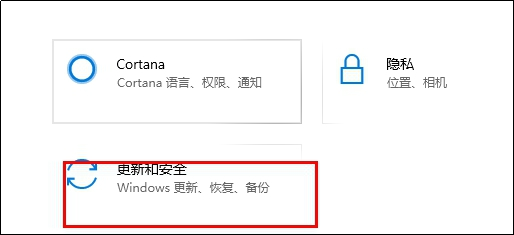
\includegraphics{001.jpg}
    \caption{第一步}
\end{figure}

\end{lstlisting}

\chapter{2020年3月2日 笔记}
\graphicspath{{note_everyday/001_20200302/picture/}}
\section{问题一:MMU学习}


1.步骤一:
\begin{figure}[h]
    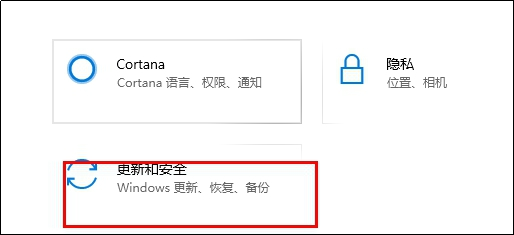
\includegraphics{001.jpg}
    \caption{第一步}
\end{figure}



\chapter{2020年3月16日 笔记}
\graphicspath{{note_everyday/001_20200316/picture/}}
\section{VOA}
%\begin{document}
\begin{lstlisting}[]
By Susan Shand
15 March 2020
Billionaire art collector David Nahmad cannot remember why he bought "Nature Morte," a small oil painting by Pablo Picasso.
Nahmad owns about 300 of Picasso's works. So, his forgetfulness is understandable.
"We bought so many Picassos now, I don't remember the... reason," Nahmad said to Associated Press reporters from his home in Monaco.
The 72-year-old started dealing art with his brothers in the 1960s, paying as little as 5,000 for pieces by Picasso and building the collection of works that made them into billionaires.
"Nature Morte" is the smallest painting Nahmad has. And it is about to belong to someone else. It will be sold to raise money for charity later this month.
Raffle tickets will be sold online and are 100 euros each. The winner of a similar Picasso raffle in 2013 was a 23-year-old worker from Pennsylvania.
Nahmad is one of the art world's most important art dealers. He will receive over 1 million for "Nature Morte." But he said the piece is worth "at least two, three times" that.
"This raffle would not have succeeded if the name was not Picasso. I tried to propose other artists' names. But it would not work, because they wanted a name that would appeal to everybody. It has to be Picasso. Picasso is the magic name," he said.
The value of Nahmad's collection is estimated to be about 3 billion. But he himself will not say what the exact value is.
"I don't think people care about the number of works, but about their quality," he said.
Nahmad said the possibility of giving up "Nature Morte" has made him look more closely at the small still life painting. It shows a newspaper and a glass of alcohol on a wood table.
"I think this painting is extremely chic," Nahmad said.
The raffle will be held in Paris on March 30. The organizers hope to sell 200,000 tickets. The money the event raises will help provide water for villagers in Cameroon, Madagascar and Morocco.
Nahmad believes that Picasso, who died in 1973, would have liked the raffling of his works to the public.
"Picasso was very generous," Nahmad said. "He wanted his art to be collected by all kinds of people, not only by the super-rich."
Nahmad's hope is that the winner of "Nature Morte" will be someone who loves the work. If not, "I will be very unhappy" and "would like to buy it back," Nahmad said.
"There's nothing worse than to own something without understanding that thing," he said.
I'm Susan Shand.
The Associated Press reported this story. Susan Shand adapted it for VOA Learning English. Ashley Thompson was the editor.
Write to us in the Comments Section or on 51VOA.COM.

\newline
%________________________________________________________________

Words in This Story
charity - n. the act of giving money, food, or other kinds of help to people who are poo

raffle – n. a contest that a group or organization uses to earn money and that involves people buying numbered tickets in exchange for a chance to win a prize

propose – v. to suggest (something, such as a plan or theory) to a person or group of people to consider

magic - n. special power, influence, or skill

chic – adj. following the current fashion or style : fashionable and appealing

generous - adj. freely giving or sharing money and other valuable things

%\end{document}
\end{lstlisting}







\end{document}



%This is 日志.

